\documentclass{standalone}
\usepackage{tikz}

\begin{document}
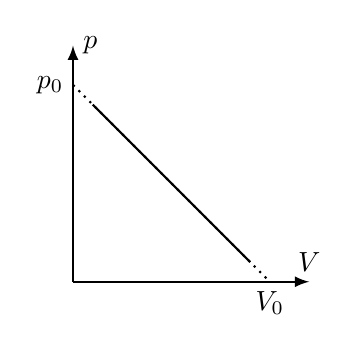
\begin{tikzpicture}
	\draw[thick, arrows={-latex}] (0,0) -- (3,0) node[above] {$V$};
	\draw[thick, arrows={-latex}] (0,0) -- (0,3) node[right] {$p$};
	\draw [thick] (0.25,2.25) -- (2.25,0.25);
	\draw[thick, dotted] (0,2.5) -- (2.5,0);
	%\draw (0,0) circle (2pt)
	\coordinate [label=left:{$p_0$}] (A) at (0,2.5);
	\coordinate [label=below	:{$V_0$}] (B) at (2.5,0);
	%\draw plot[raw gnuplot, smooth] function{set xrange[0.2:2.3]; plot 2.5-x lt 2};
\end{tikzpicture}
\end{document}